\documentclass[12pt]{book}
\usepackage{graphicx} %load EPS graphic package 
\begin{document}
\begin{figure}[!htbp]
\centering
\begin{tabular}{c}
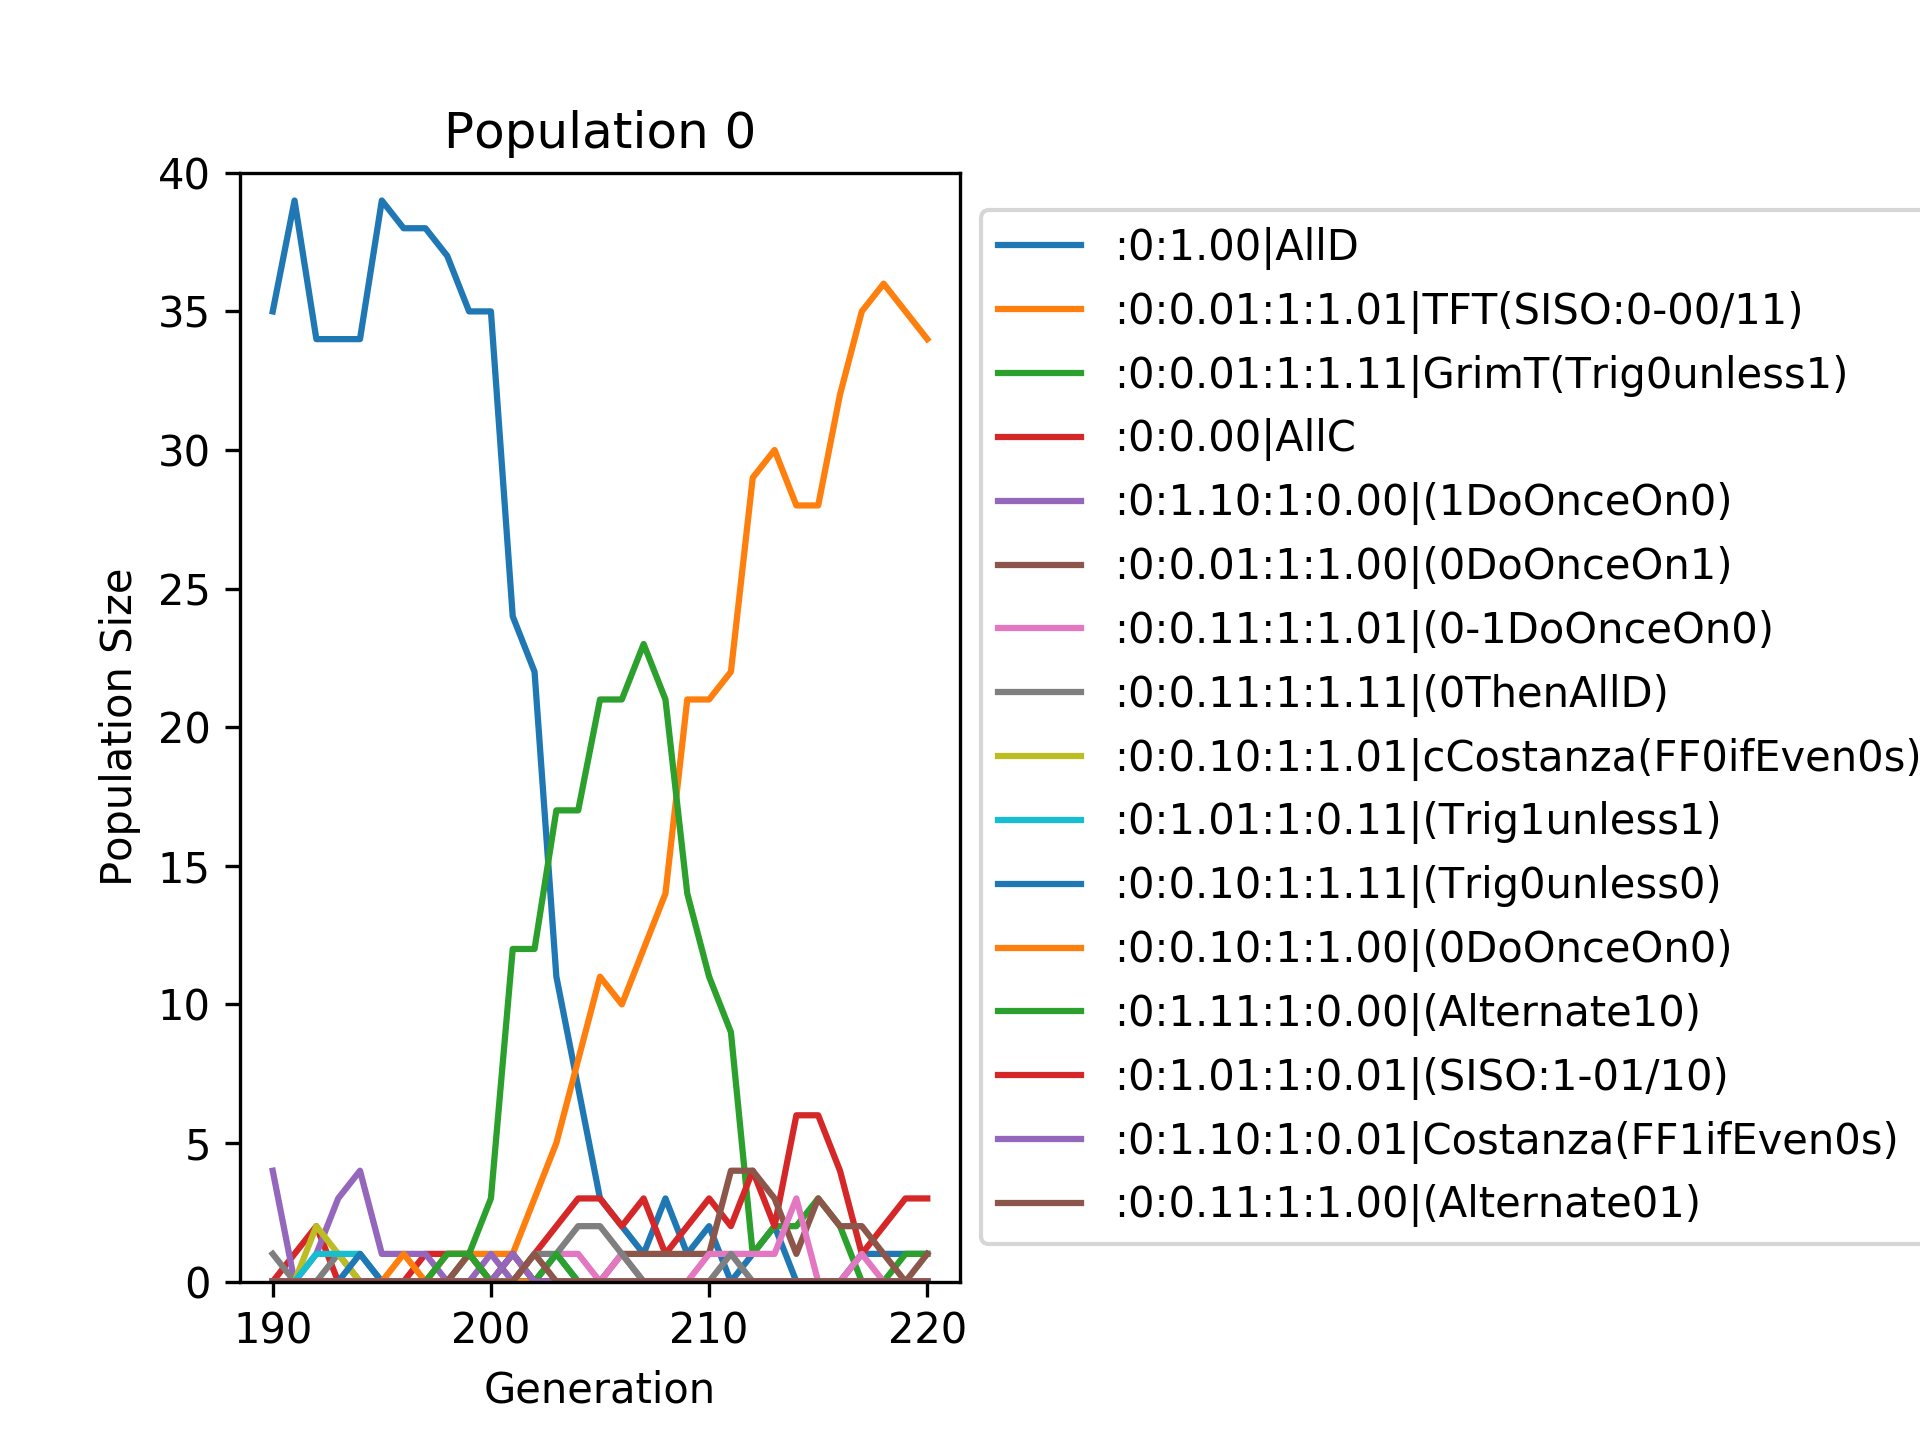
\includegraphics[height=.25\textheight]{epochP0-190-220.jpg} \\
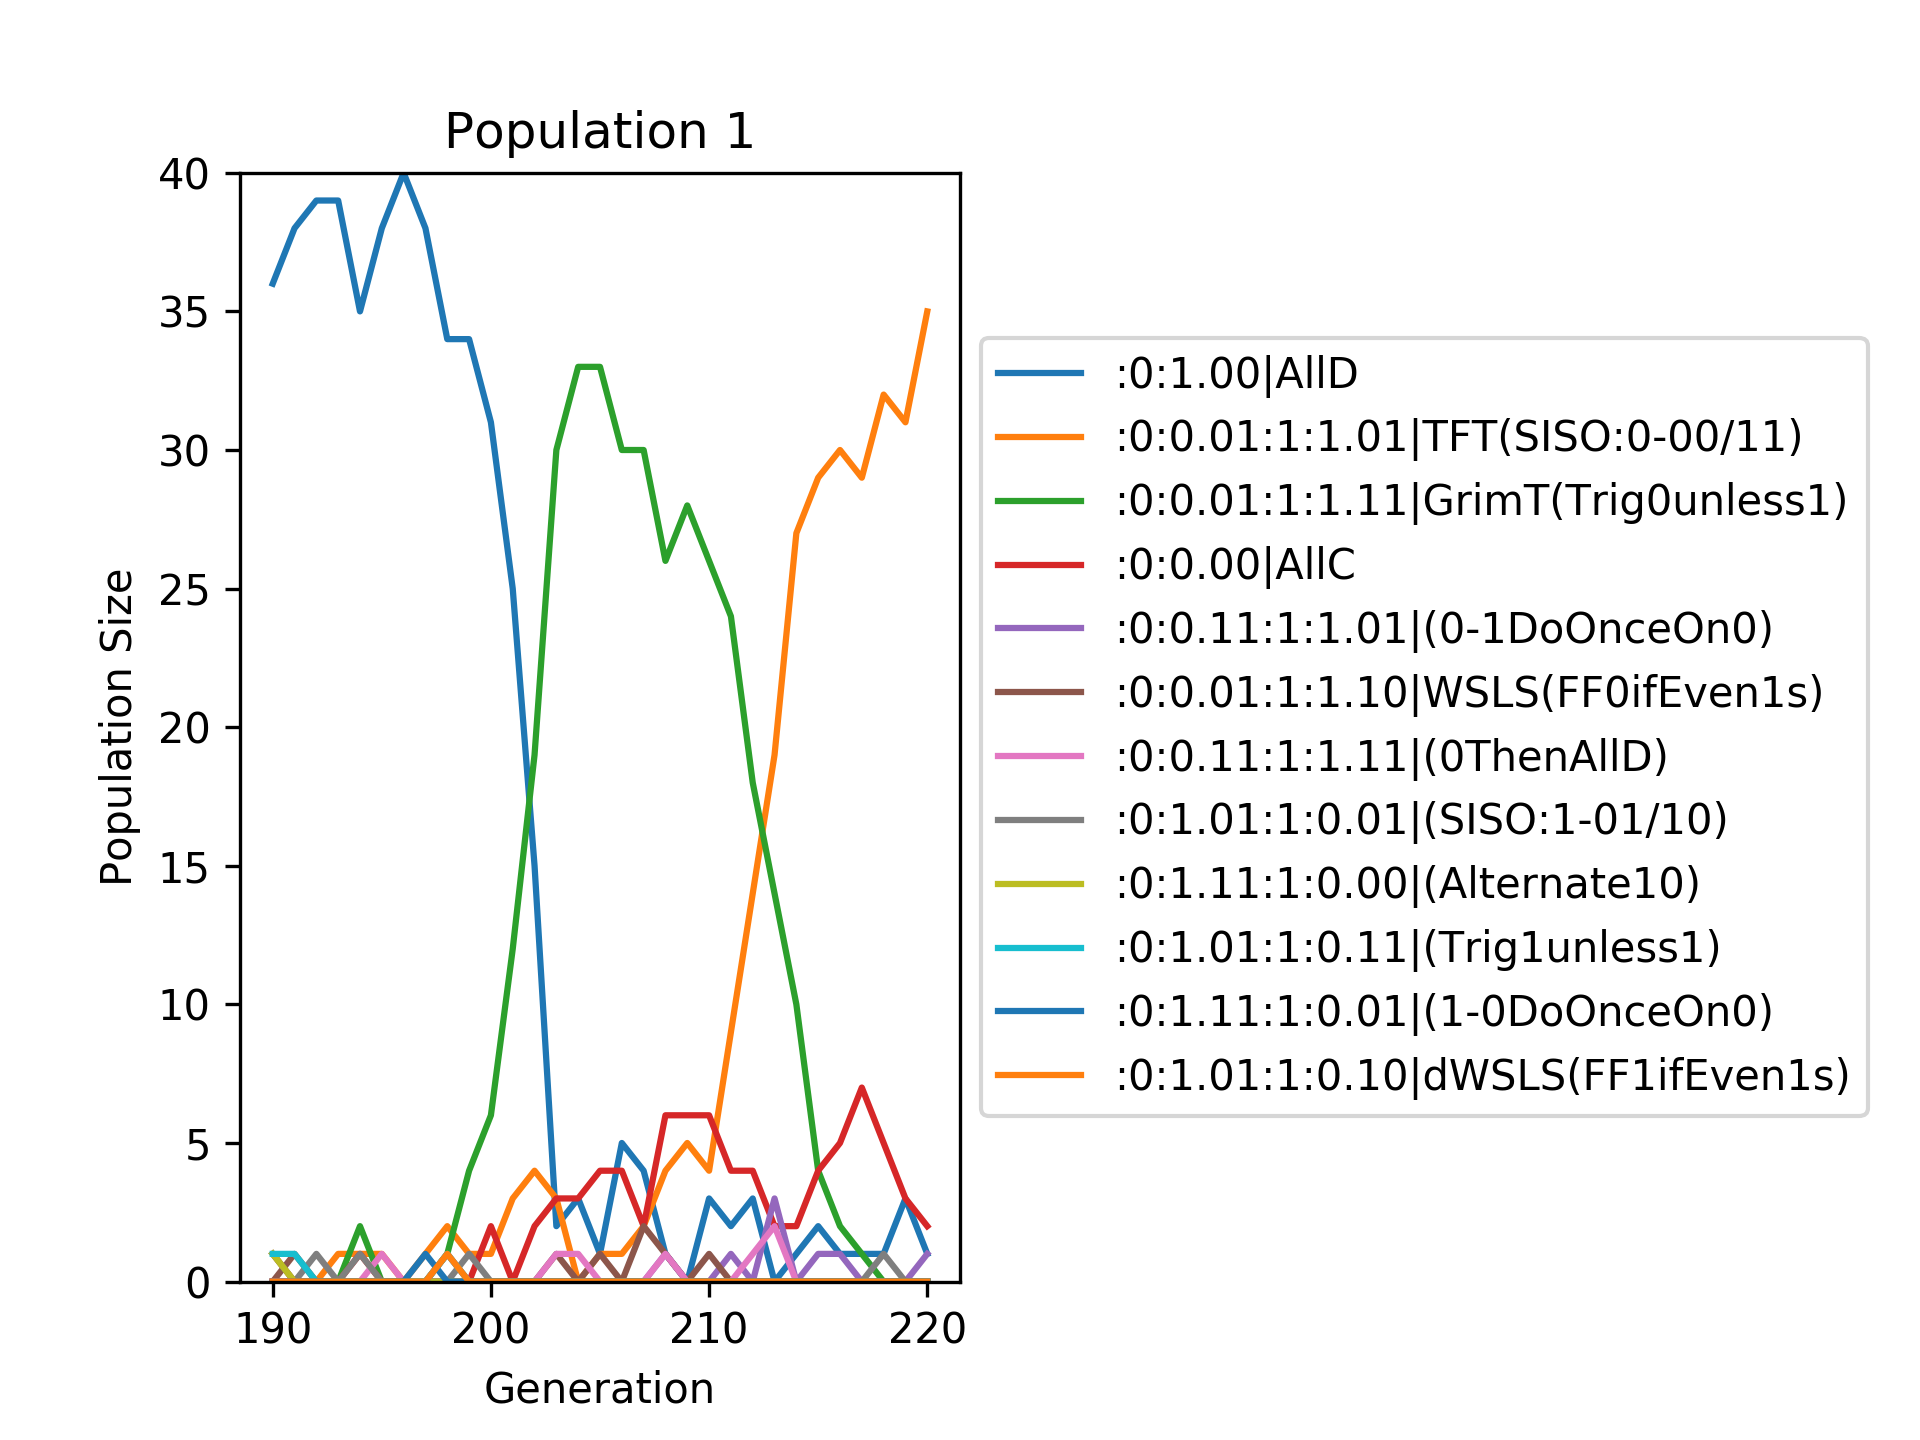
\includegraphics[height=.25\textheight]{epochP1-190-220.jpg} \\
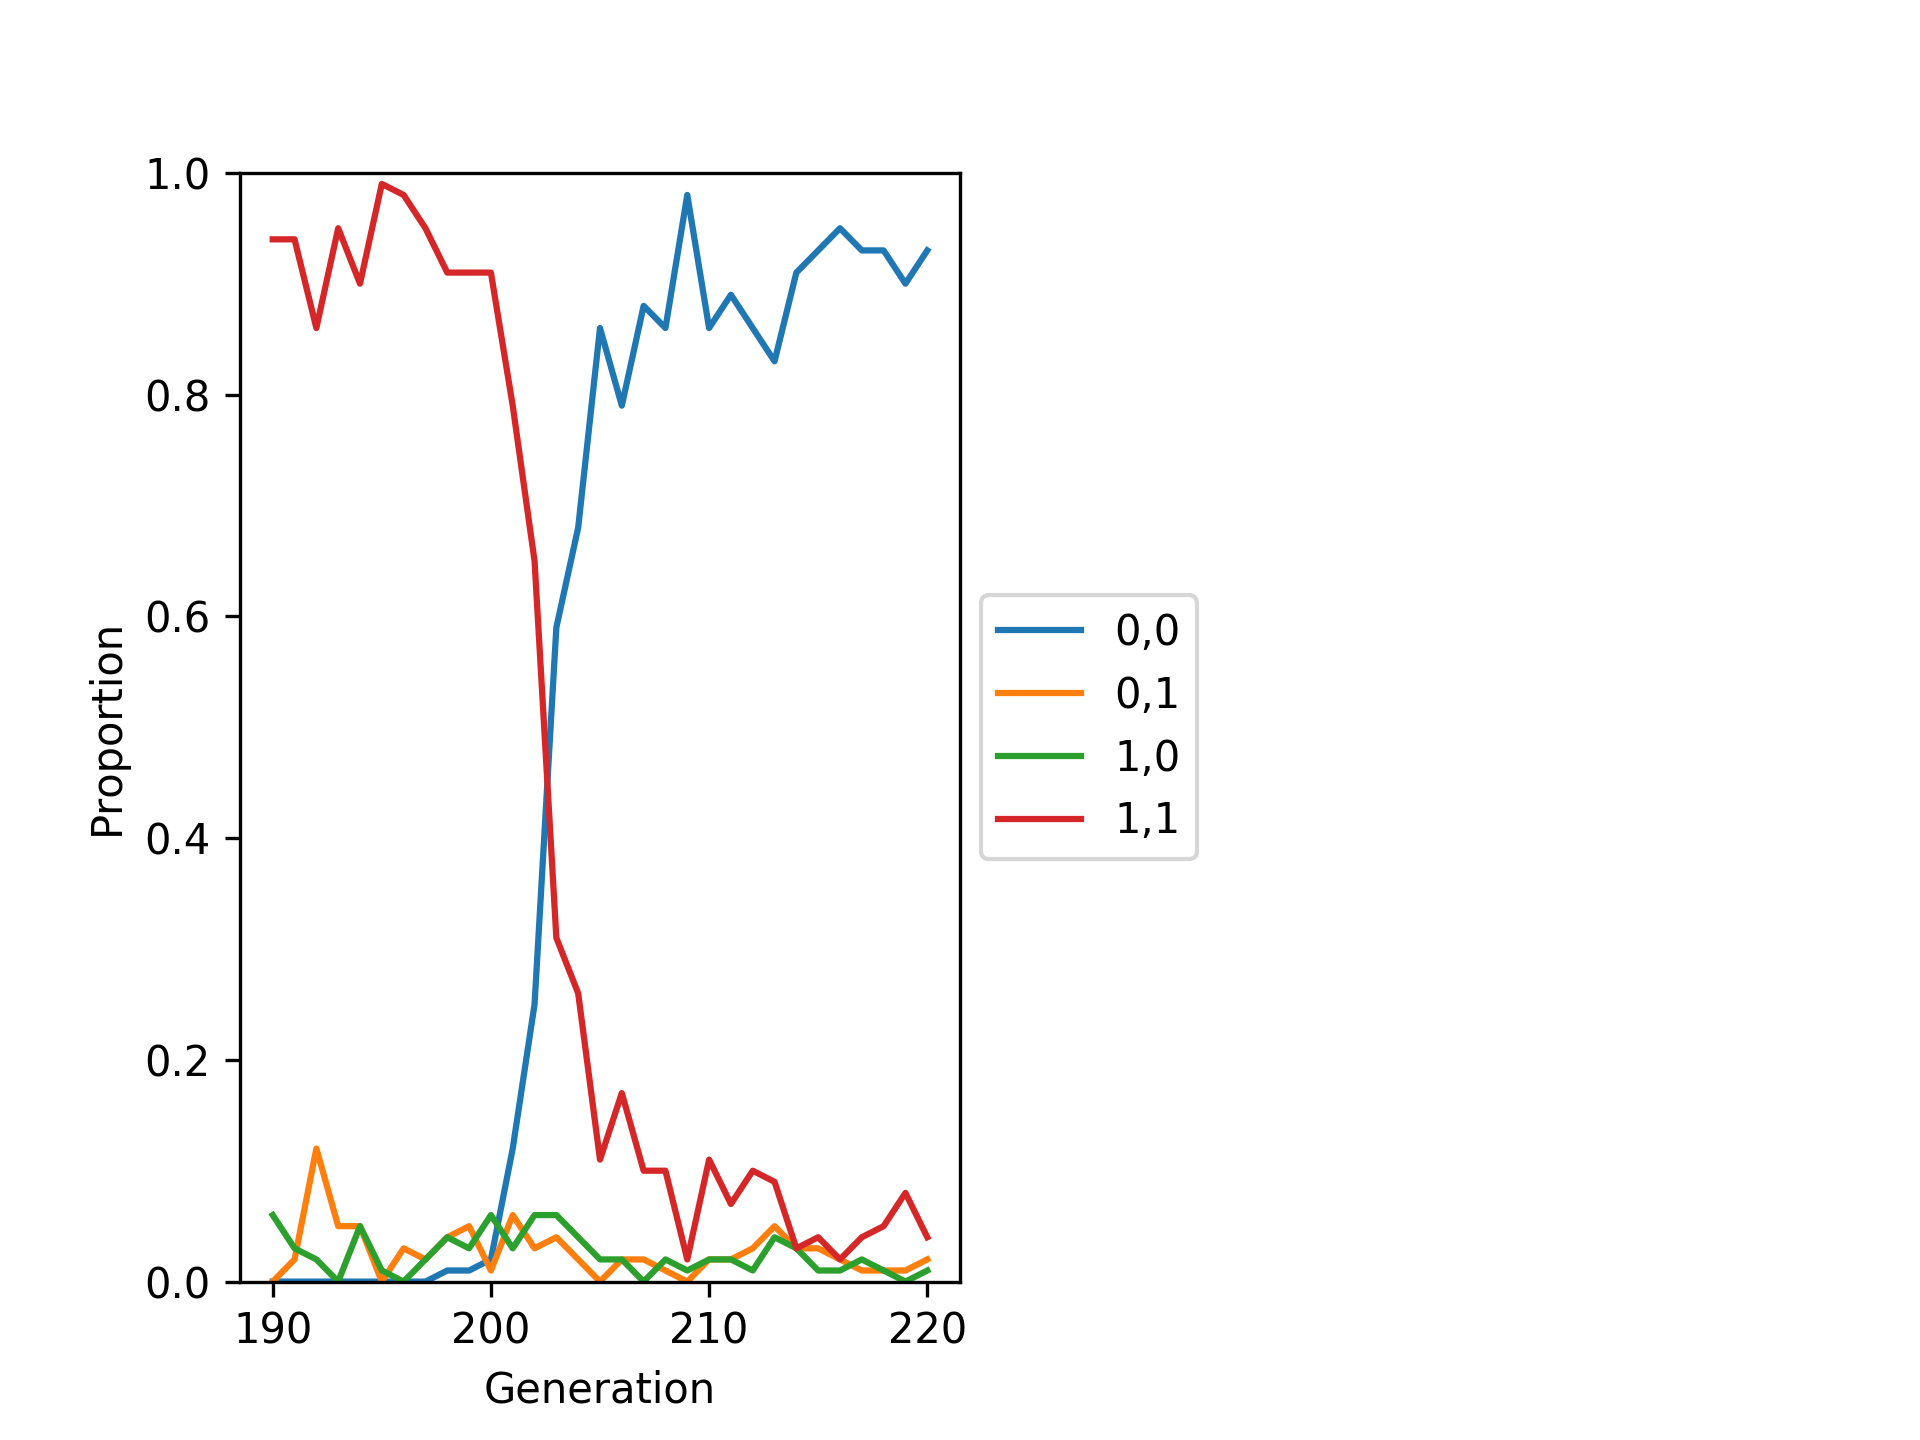
\includegraphics[height=.25\textheight]{gameplay190-220.jpg} \\
\end{tabular}
\caption[A Transiton to Cooperation]{A Transition to Cooperation in a Prisoner's
Dilemma ($T=5$,$R=4$,$P=1$,$S=0$, and 10 rounds).
In this transition the system moves from mutual defection ($\{1,1\}$) to
mutual cooperation ($\{0,0\}$) as shown in the bottom panel.  Both populations
(top two panels)
are initially dominated by Always Defect strategies.  The transition begins with
a wave of Grim Trigger strategies arising in both populations, quickly followed by a rise in Tit-For-Tat.  As the transition is completed, both populations are
dominated by Tit-For-Tat.
}
\label{fgpdtrans}
\end{figure}
\end{document}
